\documentclass[12pt]{article}

\usepackage{a4wide}
\usepackage[utf8]{inputenc}

\usepackage{graphicx}
%\usepackage{palatino}

%\pagestyle{empty}

\parindent=0pt
\begin{document}

\section{Object Features Detection}

Today's exercise is focused on implementation of simple object features.
This process will take some time and we will spend more time on this topic.

One of the possible ways in detection and classification of objects in images is using object features.
Today's lecture will consist of the following steps:

\begin{enumerate}
    \item Thresholding the image,
    \item indexing objects,
    \item computing moments and features.
\end{enumerate}

In the end, our task is to label each object in the image (Fig. \ref{fig:input}).

\subsection{Thresholding the Image}
The fist step is to separate objects in the image $f$ from the background. In our example image, this task is not so hard,
so we can apply the following thresholding criterion to each pixel in image $f$ to construct a new image $g$

\begin{equation}
g(x, y) = \left\{
\begin{array}{cc}
1, & f(x, y) > t \\
0, & \mathrm{otherwise}
\end{array}
\right.,
\end{equation}
where $t$ is a chosen threshold. There are many method to select $t$, see the text for this course.
However, in our case, we can set the threshold manually.

After this step, we have a binary image that indicates where are the objects and where is the background.

\begin{figure}[h]
\begin{centering}
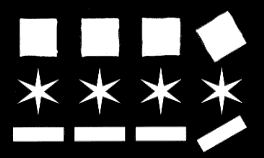
\includegraphics{train.png}
\caption{Input image.}
\end{centering}
\label{fig:input}
\end{figure}

\subsection{Indexing Objects}

In order to compute moments and features of the upcoming classification, we need to separate detected objects from the previous step.
This process is called indexing and its purpose is to distinguish between the objects in the binary image. The result of such process
is shown in Fig. \ref{fig:indexing}.

We can implement this process using a simple flood fill algorithm. In this algorithm, we go through all the pixels and if it belongs to
the objects, we label this pixel with chosen constant and recursively flood fill four neighbours with this constant too. As one might expect,
we label each object with different constant.

\begin{figure}[hb]
\begin{centering}
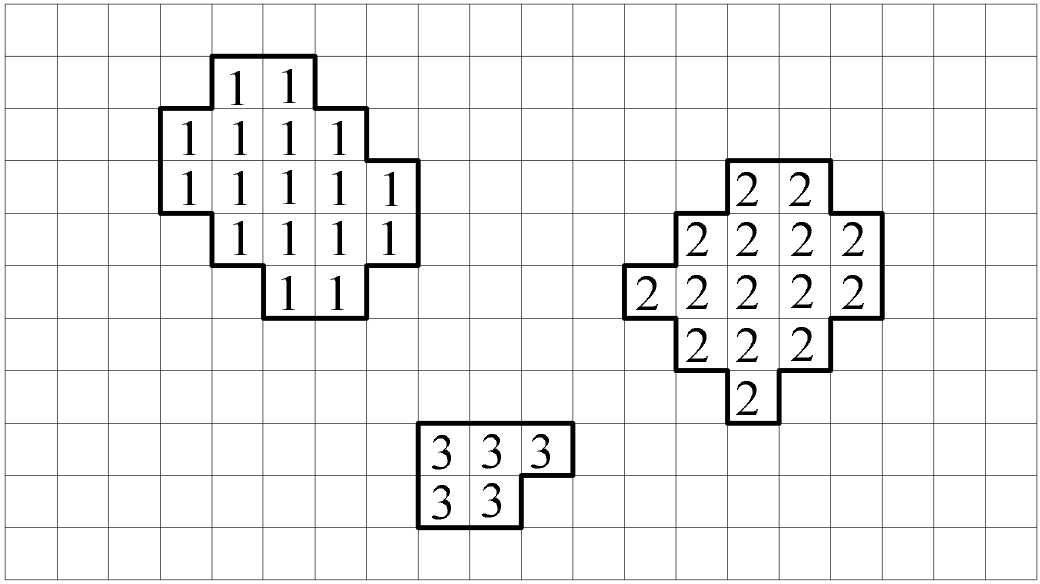
\includegraphics[width=0.4\textwidth]{indexing_scheme.png}
\caption{Indexed image.}
\end{centering}
\label{fig:indexing}
\end{figure}

\begin{figure}[hb]
\begin{centering}
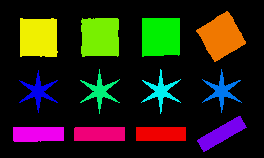
\includegraphics[width=0.4\textwidth]{indices_color.png}
\caption{Colorized indexed image for out training image. Each color represents different object index.}
\end{centering}
\label{fig:indices_color}
\end{figure}

\subsection{Computing Moments and Features}

Moments are common features that are used in object classification since they are easy to compute.

The moment that is related to the coordinate system is computed as follows

\begin{equation}
m_{p, q} = \sum\limits_{x} \sum\limits_{y} x^p y^q f(x, y) \, ,
\end{equation}
(in our case, we do not have to multiply the coordinates by the corresponding image function, since it is almost the same, see Fig. \ref{fig:input}).
\\
\\
Let us explain some important moments:
\\
\\
The \textbf{area} of an object can be computed as $m_{0, 0}$.
\\
\\
The \textbf{center of the mass} of an object:
\begin{equation}
x_t = \frac{m_{1, 0}}{m_{0, 0}}, \quad y_t = \frac{m_{0, 1}}{m_{0, 0}}
\end{equation}

The \textbf{perimeter} of an object may be computed using a simple algorithm that scans each pixel of the object and if the four neighbour of the pixel
contains the same values as the central pixel than this pixel does not contribute to the perimeter, otherwise it does.

\end{document}

